\documentclass[a4paper, 11pt]{article}
\usepackage{comment}
\usepackage{lipsum} 
\usepackage{fullpage} %cambiar margen
\usepackage[a4paper, total={7in, 10in}]{geometry}

\usepackage{amssymb,amsthm} 
\usepackage{amsmath}
\newtheorem{theorem}{Theorem}
\newtheorem{corollary}{Corollary}
\usepackage{graphicx}
\usepackage{tikz}
\usetikzlibrary{arrows}
\usepackage{verbatim}
%\usepackage[numbered]{mcode}
\usepackage{float}
\usepackage{tikz}
\usetikzlibrary{shapes,arrows}
\usetikzlibrary{arrows,calc,positioning}
\usepackage{mathpazo} %tipo de letra 
\usepackage[utf8]{inputenc} %codificación
\usepackage[T1]{fontenc} %digitación de tildes y ñ
\usepackage[spanish]{babel} %paquete de soporte español

\tikzset{
	block/.style = {draw, rectangle,
		minimum height=1cm,
		minimum width=1.5cm},
	input/.style = {coordinate,node distance=1cm},
	output/.style = {coordinate,node distance=4cm},
	arrow/.style={draw, -latex,node distance=2cm},
	pinstyle/.style = {pin edge={latex-, black,node distance=2cm}},
	sum/.style = {draw, circle, node distance=1cm},
}
\usepackage{xcolor}
\usepackage{mdframed}
\usepackage[shortlabels]{enumitem}
\usepackage{indentfirst}
\usepackage{hyperref}

\usepackage{listings}
\lstset{literate=
  {á}{{\'a}}1
  {é}{{\'e}}1
  {í}{{\'i}}1
  {ó}{{\'o}}1
  {ú}{{\'u}}1
  {Á}{{\'A}}1
  {É}{{\'E}}1
  {Í}{{\'I}}1
  {Ó}{{\'O}}1
  {Ú}{{\'U}}1
  {ñ}{{\~n}}1
  {ü}{{\"u}}1
  {Ü}{{\"U}}1
}

\lstdefinestyle{customc}{
  belowcaptionskip=1\baselineskip,
  breaklines=true,
  frame=L,
  xleftmargin=\parindent,
  language=Python,
  showstringspaces=false,
  basicstyle=\footnotesize\ttfamily,
  keywordstyle=\bfseries\color{green!40!black},
  commentstyle=\itshape\color{purple!40!black},
  identifierstyle=\color{blue},
  stringstyle=\color{orange},
}

\lstdefinestyle{customasm}{
  belowcaptionskip=1\baselineskip,
  frame=L,
  xleftmargin=\parindent,
  language=[x86masm]Assembler,
  basicstyle=\footnotesize\ttfamily,
  commentstyle=\itshape\color{purple!40!black},
}

\lstset{escapechar=@,style=customc}



\renewcommand{\thesubsection}{\thesection.\alph{subsection}}

\newenvironment{problem}[2][Ejercicio]
{ \begin{mdframed}[backgroundcolor= red!50] \textbf{#1 #2} \\}
	{  \end{mdframed}}

% Define solution environment
\newenvironment{solution}
{\textcolor{blue}{\textbf{\textit{Solución:\\\noindent}}}}


\renewcommand{\qed}{\quad\qedsymbol}

% \\	
\begin{document}
	\noindent
	%%%%%%%%%%%%%%%%%%%%%%%%%%%%%%%%%%%%
	
	\begin{minipage}[b][1.2cm][t]{0.8\textwidth}
		\large\textbf{César Isaí García Cornejo} \hfill \textbf{Tarea 1}  \\
		cesar.cornejo@cimat.mx \hfill \\
		\normalsize Ciencia de Datos \hfill Semestre 3\\
	\end{minipage}
	
	\hspace{14.4cm}
	\begin{minipage}[b][0.03cm][t]{0.12\linewidth}
		
		\vspace{-2.2cm}
		%%%La Ruta depeendera de donde este alojado el main y la imagen
		
\includegraphics[scale=0.3]{Images/EscudoCimat.png}
	\end{minipage}
	
	\noindent\rule{7in}{2.8pt}
	
	%%%%%%%%%%%%%%%%%%%%%
	%%%%%%%%%%%%%%%%%%%%%%%%%%%%%%%%%%%%%%%%%%%%%%%%%%%%%%%%%%%%%%%%%%%%%%%%%%%%%%%%%%%%%%%%%%%%%%%%%%%%%%%%%%%%%%%%%%%
	% Problem 1
	%%%%%%%%%%%%%%%%%%%%%%%%%%%%%%%%%%%%%%%%%%%%%%%%%%%%%%%%%%%%%%%%%%%%%%%%%%%%%%%%%%%%%%%%%%%%%%%%%%%%%%%%%%%%%%%%%%%%%%%%%%%%%%%%%%%%%%%%
	\setlength{\parskip}{\medskipamount}
	\setlength{\parindent}{0pt}
 
\begin{problem}{1}
Considere tres poblaciones Poisson, con parámetros $\lambda_1 = 10$, $\lambda_2 = 15$, $\lambda_3 = 20$ respectivamente.
\begin{enumerate}
    \item Establezca la regla óptima de clasificación, basandose en una sola observación, $x$.
    \item Calcule la probabilidad de error asociado a esta regla óptima.
    \item Escriba un programa (R o Python) para validar, vía simulación, el nivel de error encontrado en el inciso anterior.
\end{enumerate}

\end{problem}
	
\begin{solution}
    \begin{enumerate}
        \item Por el siguiente Teorema construimos la regla óptima para la clasificación de interes.

        \textbf{Teorema:} 
        
        Supongamos que $Y \in \mathcal{Y} = \{1,...,K\}$. La regla óptima es
        \begin{align}
            g(x) =& argmax_k \mathbb{P}(Y=k|X=x), \nonumber\\
             =&argmax_k \pi_k f_k(x) \label{1.01}
        \end{align}
        donde 
        \begin{align*}
            \mathbb{P}(Y=k|X=x) = \frac{f_k(x)\pi_k}{\sum_r f_r(x)\pi_r},
        \end{align*}
        $\pi_r = \mathbb{P}(Y=r)$, $f_r(x)= f(x|Y=r)$ y $argmax_k$ significa ``el valor de $k$ que maximiza la expresión.''

        De esta forma, notamos que las tres poblaciones están \textit{dispersas} en $\mathbb{N} \cup \{0\}$. Como la media de cada población es su propio parámetro entonces las tres poblaciones están ordenadas en la recta real. Con la única observación $x \in \mathbb{R}$ y considerando las barreras de decisión (suponiendo que $\pi_1 = \pi_2 = \pi_3 = 1/3$ )
        \begin{align*}
            \mathbb{P}(X=x|Y=1) = \mathbb{P}(X=x|Y=2), \:\:\:\:\:   \mathbb{P}(X=x|Y=2) = \mathbb{P}(X=x|Y=3)
        \end{align*}
        Manipulando tenemos
        \begin{align*}
            \mathbb{P}(X=x|Y=1) &= \mathbb{P}(X=x|Y=2), \\  
            \frac{\lambda_1^x}{x!}e^{-\lambda_1} &= \frac{\lambda_2^x}{x!}e^{-\lambda_2},\\
            \left (\frac{\lambda_1}{\lambda_2}  \right )^x &= e^{\lambda_1 - \lambda_2} \\
            x \log \left (\frac{\lambda_1}{\lambda_2}  \right ) &= \lambda_1 - \lambda_2, \\
            x &= \frac{\lambda_1 - \lambda2}{ \log(\lambda_1) - \log(\lambda_2)} \\
            x & \approx 12.33
        \end{align*}
        Análogamente, 
        \begin{align*}
            \mathbb{P}(X=x|Y=2) &= \mathbb{P}(X=x|Y=3),\\
            x &\approx 17.38
        \end{align*}
        De está forma, podemos construir $g(x) \rightarrow \mathcal{Y}$ partiendo el intervalo como
        \begin{align*}
            g(x) = 
            \left\{\begin{matrix}
            1 & &x\leq 12.33 \\ 
            2 & &12.33 < x \leq 17.38 \\
            3 & &x\geq 17.38
            \end{matrix}\right. 
        \end{align*}
        como $x\in \mathbb{N}\cup \{0\}$ se obtiene finalmente
        \begin{align}
            g(x) = 
            \left\{\begin{matrix}
            1 & &x\leq 12 \\ 
            2 & & 13 \leq x \leq 17 \\
            3 & &x\geq 18
            \end{matrix}\right. 
        \end{align}
        la regla de clasificación óptima.

        \item Calculemos ahora la probabilidad de error $\mathbb{P}(g(X)\neq Y)$ de la función $g(X)$ asociada.
        \begin{align*}
            \mathbb{P}(g(X)\neq Y) &= 1 - \mathbb{P}(g(X) = Y) \\
            &= 1 - \mathbb{P}(g(X) = 1| Y = 1 )\pi_1 - \mathbb{P}(g(X) = 2| Y = 2 )\pi_2 -\mathbb{P}(g(X) = 3| Y = 3 )\pi_3 \\
            &= 1 - \frac{1}{3}\left ( \mathbb{P}(X\leq 12|Y=1) +  \mathbb{P}(13 \leq X \leq 17|Y=2) + \mathbb{P}(X\geq 18|Y = 3)\right ),\\
            &= \text{0.3414}
        \end{align*}
        donde las cuentas se obtuvieron computacionalmente con el \href{https://colab.research.google.com/drive/1-OkL9CyO0Sanx695uaE9ssM8Y0RIWvLF?usp=sharing}{código} adjunto.

        \item Para poder obtener vía simulación una probabilidad nos basaremos en la ley de grandes números. Es decir tomaremos la proporción de errores de clasificación obtenidos bajo $m$ iteraciones. Seleccionando una de las tres poblaciones posibles con sus respectivos parámetros y simulando una variable poisson, podemos entonces usar $g(x)$ para clasificar la realización $x$ en la simulación. Tomando $m$ relativamente grande, este debe converger a la probabilidad de error de la regla de clasificación.

        Dicha simulación se implemento en Python. Para obtener una elección al azar de las clases usamos el comando

\begin{lstlisting}[language = Python]
    r = random.choice(clases) #Seleccionar clase
\end{lstlisting}

        Luego con scipy se simula la Poisson con su respectivo parámetro. Así podemos entonces usar la regla de clasificación para contar los errores que produce, mostrado en el condicional que adjunta a una lista una variable booleana que es True si está mal clasificado. Finalmente cuenta el promedio de errores en dicha lista.

\begin{lstlisting}[language = Python]
for i in range(m):
    r = random.choice(clases)
    x = poisson.rvs(lamda[r-1])
    if r == 1:
        error.append(x >= 13)
    elif r == 2:
        error.append( (x <= 12) or (x>= 18))
    elif r == 3:
        error.append((x <= 17))

print("La proporción de errores es: ", sum(error)/len(error))
\end{lstlisting}

El resultado obtenido por está simulación nos dice que
\begin{align}
    \mathbb{P}(g(X)\neq Y) \approx 0.3421
\end{align}
que es bastante similar al obtenido analíticamente. Enfatizo que el enlace al código detallado se encuentra \href{https://colab.research.google.com/drive/1-OkL9CyO0Sanx695uaE9ssM8Y0RIWvLF?usp=sharing}{\color{blue}aquí}

    \end{enumerate}

   
\end{solution}


\begin{problem}{2}
Descargue la base de datos llamada Wine.
\begin{enumerate}
    \item Basados en las características químicas de los vinos, construya un clasificador para determinar el origen de los mismos.
    \item ?` Cuántos vinos están mal clasificados por este clasificador?
\end{enumerate}

\end{problem}
	
\begin{solution}
    \begin{enumerate}
        \item Vemos de la base de datos que tenemos 14 columnas de las cuales la primera es la columna de la clase a la que pertenece cada vino. Luego las restantes 13 columnas serán las que pertenecen a los atributos de cada vino. 
        En la Fig~\ref{Fig01} mostramos la cabeza de dicha base de datos.
        
         \begin{figure}[H]
             \centering
             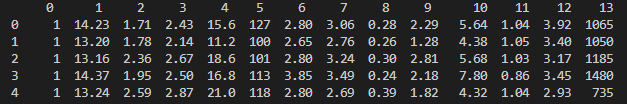
\includegraphics[width = 13 cm]{Images/datos.png}
             \caption{Primeros datos en wine}
             \label{Fig01}
         \end{figure}
     
        Para hacer un modelo de clasificación optamos por construirlo con el clasificador de Bayes Gaussiano. Primeramente, se requiere partir la base de datos en la tradicional particion de datos de prueba y datos de entrenamiento. Para ello y con la paqueteria sklearn podemos hacer la partición con el siguiente comando
     
        \begin{lstlisting}
from sklearn.model_selection import train_test_split
X_train, X_test, y_train, y_test = train_test_split(X, y, test_size=0.4, random_state=1)
        \end{lstlisting}
     
        Ahora, implementamos el modelo naive Bayes Gaussiano con el comando 
    
        \begin{lstlisting}
from sklearn.naive_bayes import GaussianNB
gnb = GaussianNB()
gnb.fit(X_train, y_train)
        \end{lstlisting}
        lo que concluye la construcción del modelo.

        \item Para medir la precisión del modelo construido hacemos uso de la predicción que tienen los datos de prueba y comparamos con las verdaderas clasificaciones. Esto se obtiene con el comando siguiente
        \begin{lstlisting}
# making predictions on the testing set
y_pred = gnb.predict(X_test)
        \end{lstlisting}
        
        Imprimendo el resultado dado vinos mal clasificados por el modelo propuesto 
        \begin{lstlisting}
from sklearn import metrics
print("Gaussian Naive Bayes model accuracy(in %):", metrics.accuracy_score(y_test, y_pred)*100)
        \end{lstlisting}
        se obtiene que la proporción de vinos mal clasificados es de 98.61 \% que lo hace un excelente clasificador.

    \end{enumerate}

    El código en detalle se encuentra \href{https://colab.research.google.com/drive/1dJkJfHKAnInkXYZjEc13jcOcUDfCJWdL?usp=sharing}{\color{blue}aquí}.

\end{solution}

\end{document}